\documentclass[12pt]{article}

% PACKAGES
\usepackage{graphicx, amsmath, amssymb, amsfonts, mathtools, mathrsfs, color}
\usepackage{comment, enumerate, tabularx}
\usepackage{natbib, hyperref, url}
\usepackage[margin=1in]{geometry}
%\usepackage[justification=RaggedRight]{caption}

%%%%%%%%%%%%%%%%%%%%%%%%%%%%%%%%%%%%%%
%% LATEX DEFINITIONS
%%%%%%%%%%%%%%%%%%%%%%%%%%%%%%%%%%%%%%

% Basic editing
\newcommand{\tocite}{{\color{blue}(to cite)}}
\newcommand{\vsp}[1]{\vspace{#1 pc} \noindent}
\newcommand{\np}{\newpage \noindent}
% Derivatives
\newcommand{\pd}[2]    { \frac{\partial #1} {\partial #2} }
\newcommand{\ppd}[2]  { \frac{\partial^2 #1}{{\partial #2}^2} }
\newcommand{\pdi}[2] { {\partial_#2} #1 }
\newcommand{\td}[2] { \frac{d #1} { d #2 } }
\newcommand{\grad}{\nabla}
\newcommand {\Lap} {\grad^2}
% Vectors and operators
\newcommand{\bvec}[1]{\ensuremath{\boldsymbol{#1}}}
\newcommand{\abs}[1]{\left| #1 \right|}
\newcommand{\norm}[1]{\left\| #1 \right\|}
\newcommand{\mean}[1]{\left< #1 \right>}
\newcommand{\eps}{\varepsilon}

% Experimental parameters
\newcommand{\lamm}{\lambda^{-}}
\newcommand{\lamp}{\lambda^{+}}
\newcommand{\hm}{h^{-}}
\newcommand{\hp}{h^{+}}
\newcommand{\etastd}{\eta_{\text std}}
% Theory for truncated KdV and stat mech
\newcommand{\uhat}{\hat{u}}
\newcommand{\RR}{\mathbb{R}}
\newcommand{\Real}{\text{Re}}
\newcommand{\Fspace}{\mathscr{F}_{\Lambda}}
\newcommand{\Proj}{P_{\Lambda}}
\newcommand{\sumk}{\sum_{k=1}^{\Lambda}}
\newcommand{\sumn}{\sum_{n=1}^{N}}
\newcommand{\uDir}{u_{\text{Dir}}}
\newcommand{\Gibbs}{\mathcal{G}}



% Dashed integral
\def\Xint#1{\mathchoice
   {\XXint\displaystyle\textstyle{#1}}%
   {\XXint\textstyle\scriptstyle{#1}}%
   {\XXint\scriptstyle\scriptscriptstyle{#1}}%
   {\XXint\scriptscriptstyle\scriptscriptstyle{#1}}%
   \!\int}
\def\XXint#1#2#3{{\setbox0=\hbox{$#1{#2#3}{\int}$}
     \vcenter{\hbox{$#2#3$}}\kern-.5\wd0}}
\def\ddashint{\Xint=}
\def\dashint{\Xint-}
\newcommand{\intt}{\dashint}%_0^{2 \pi}}
\newcommand{\dx}{\, dx}


%%%%%%%%%%%%%%%%%%%%%%%%%%%%%%%%%%%%%%
%% TITLE
%%%%%%%%%%%%%%%%%%%%%%%%%%%%%%%%%%%%%%
\begin{document}
\title{Deterministic and statistical truncated KdV models for anomalous waves induced by abrupt depth change}
\author{}
\maketitle


%%%%%%%%%%%%%%%%%%%%%%%%%%%%%%%%%%%%%%
%% Mathematical Preliminaries
%%%%%%%%%%%%%%%%%%%%%%%%%%%%%%%%%%%%%%
\section{Mathematical preliminaries}

\subsection{Truncated Fourier series}

We will be dealing with the truncated KdV equation (TKDV). 
Consider a real-valued function $u(x): [0, 2\pi] \to \RR$ given by a truncated Fourier series
\begin{equation}
u(x) = \sum_{k= -\Lambda}^{\Lambda} \uhat_k e^{i k x}	\qquad \text{for } 0 \le x \le 2\pi
\end{equation}
where
\begin{equation}
\uhat_k = \intt u(x) e^{-i k x} \dx
\end{equation}
Above, and throughout the paper, we use the notation
\begin{equation}
\intt \cdot \, \dx  = \frac{1}{2\pi} \int_0^{2 \pi} \cdot \, \dx
\end{equation}
We will be dealing with zero-momentum functions
\begin{equation}
M = \intt u(x) \dx = 0
\end{equation}
Let $\Fspace$ denote the space of all zero-momentum functions that can be represented by the above truncated Fourier Series (with maximum wavenumber $\Lambda$).

Since any element $u \in \Fspace$ is real valued and has zero momentum, it can be written as
\begin{equation}
u(x) = \sumk \uhat_k e^{i k x} + \uhat_k^{*} e^{-i k x} 
= 2 \Real \sumk \uhat_k e^{i k x}
\end{equation}
This implies that $\dim(\Fspace) = \Lambda$ as a complex vector space (or the dimension of the equivalent real vector space is $2\Lambda$).
For any $u \in \Fspace$, we introduce the energy
\begin{equation}
E = \frac{1}{2} \intt \Proj(u^2) \dx = \sumk \abs{\uhat_k}^2
\end{equation}
where $\Proj$ is the projection onto $\Fspace$.
In order to define the Hamiltonian for TKDV, we introduce the following components
\begin{equation}
H_3 = \frac{1}{6} \intt \Proj(u^3) \dx \qquad H_2 = \frac{1}{2} \intt \Proj(u_x^2) \dx
\end{equation}
We note that $H_3$ can be written explicitly in Fourier space as \cite{abramov2003hamiltonian} 
\begin{equation}
\label{H3dirsum}
H_3 = \frac{1}{6} \sum_{\substack{ k_1 + k_2 + k_3 = 0 \\ \abs{k_1}, \abs{k_2}, \abs{k_3} \le \Lambda}}\uhat_{k_1} \uhat_{k_2} \uhat_{k_3}
\end{equation}

\subsection{Some useful estimates/bounds for $H_2$ and $H_3$}

Since we examine the statistical mechanics of TKDV, it is valuable to have some a priori bounds and estimates for the components of the Hamiltonian, $H_2$ and $H_3$. In this section, we frequently appeal to the idea of an equipartition of energy among all the modes. For energy $E_0$, if the equipartition holds, then
\begin{equation}
\abs{u_k} = \sqrt{\frac{E_0}{\Lambda}} \qquad \text{for } k=1,\cdots,\Lambda
\end{equation}
We might expect equipartition of energy to hold, for example, in the case of long-time averages or ensemble averages (appealing to ergodicity).

\subsubsection{Expected value of $H_2$ given $E=E_0$}

First, we consider $H_2$. In Fourier space, $u_x$ is represented as
\begin{equation}
u_x(x) = 2 \Real \sumk i k \uhat_k e^{i k x}
\end{equation}
Thus, for equipartitioned energy, we have
\begin{equation}
H_2 = \sumk \abs{k \uhat_k}^2 = \frac{E_0}{\Lambda} \sumk k^2 = \frac{E_0}{6} (\Lambda+1)(2 \Lambda+1) \sim \frac{E_0 \Lambda^2}{3} \text{for } \Lambda \gg 1
\end{equation}
The above provides a useful estimate for the expected value of $H_2$ (to test the numerics for example).

\subsubsection{Upper bound on $H_3$ given $E=E_0$}

Next, consider $H_3$. By the symmetry of the cubic form, the expected value of $H_3$ is zero. However, to sample from Gibbs measures with non-vanishing inverse temperatures using an acceptance/rejection based algorithm, we will need to estimate the maximum allowed value of $H_3$ on the hypersphere of fixed energy $E = E_0$ so that the acceptance rate can be normalized. Note that the set $E=E_0$ is compact and therefore a maximum is guaranteed to exist. A reasonable guess for function that maximizes $H_3$ is something approximating a Dirac delta function, which naturally motivates the Dirichlet kernel
\begin{equation}
\label{Dkern}
\uDir(x) = \sqrt{\frac{E_0}{\Lambda}}\sumk e^{i k x}
\end{equation}
We can compute $H_3(\uDir)$ by using the direct summation formula \eqref{H3dirsum}. Since $\uhat_k = \sqrt{E_0/\Lambda}$, each term in this sum takes the value $(E_0/\Lambda)^{3/2}$, and so we simply need to count the number of terms present in this sum. A careful counting (being sure to dismiss any terms in which one of $k_1, k_2, k_3$ is zero or one of these terms exceeds $\Lambda$) gives
\begin{equation}
\label{H3Dir}
H_3(\uDir) = \frac{1}{2} E_0^{3/2} (\Lambda^{1/2} - \Lambda^{-1/2})
\end{equation}
Certainly, it must be that
\begin{equation}
\max H_3 \ge H_3(\uDir) 
\end{equation}
My conjecture is that
\begin{equation}
\max H_3 = H_3(\uDir) 
\end{equation}
or at least that this relationship holds asymptotically for $\Lambda \gg 1$.
Preliminary numerical tests seem to support this conjecture for tested values $\Lambda = 6, 8, 10, 20$. In fact, the maximum of $H_3$ encountered over about $10^6$ samples is usually significantly smaller than the value predicted in \eqref{H3Dir}. However, for $\Lambda = 4$, my tests encounter values of $H_3$ slightly larger than the predicted value.

Maximizing $H_3$ is perhaps more straightforward in physical space, where we discretize the interval $[0, 2 \pi)$ with 
\begin{equation}
x_n = \frac{2 \pi (n-1)}{N} \quad \text{for } n=1,\cdots,N
\end{equation}
where
\begin{equation}
N = 2 \Lambda \text{ or  } 2 \Lambda +1
\end{equation}
Both are valid choices for using standard real FFT packages.
%$x_n = 2 \pi (n-1)/N$ for $n=1,\cdots,N$, and $N$ is either $2 \Lambda$ or $2 \Lambda + 1$ (both are valid choices for using standard real FFT packages). 
In physical space, we have
\begin{equation}
\label{H3phys}
H_3 = \frac{1}{6} \intt \Proj (u^3) \dx \approx \frac{1}{6N} \sumn u_n^3
\end{equation}
The second relationship is only an approximation because de-aliasing would be required to make the right-hand side exactly equal to \eqref{H3dirsum}. Nonetheless, let us proceed with the estimate. For fixed energy, $E=E_0$, we require
\begin{equation}
E_0 = \intt \Proj(u^2) \dx = \frac{1}{N} \sumn u_n^2
\end{equation}
(I believe the above holds with no approximation being made due to the discrete Parseval identity) 

Clearly, a maximizer of the right-hand-side of \eqref{H3phys} subject to $M=0$ and fixed $E=E_0$ is an approximate Dirac delta function --- i.e. a function with one extreme positive value, and the rest equal negative values,
\begin{align}
& w_1 = \sqrt{2 E_0 (N-1)}		\\
& w_n = -\sqrt{\frac{2 E_0}{N-1}}	\qquad \text{for } n \ne 1
\end{align}
This function is a maximizer because any slight modification (subject to keeping $M=0$ and $E=E_0$) would reduce the value of $H_3$.
Calculating the discrete Fourier transform of this function directly gives
\begin{align}
& \hat{w}_0 = 0	\\
& \hat{w}_k = \sqrt{\frac{2 E_0}{N-1}} \qquad \text{for } k \ne 1
\end{align}
Notice that if we choose $N = 2\Lambda + 1$, then our delta-function in physical space corresponds exactly to the Dirichlet kernel, $w(x) = \uDir(x)$. Now, if we calculate $H_3(w)$ purely in physical space using the approximation in \eqref{H3phys}, we get
\begin{equation}
H_3(w) = \frac{\sqrt{2} E_0^{3/2}}{3} \left( \frac{N-2}{\sqrt{N-1}} \right)
\end{equation}
Taking $N = 2\Lambda + 1$ gives
\begin{equation}
\label{H3physest}
H_3(w) = \frac{2 E_0^{3/2}}{3} \left( \Lambda^{1/2} - \Lambda^{-1/2} \right)
\end{equation}
So while \eqref{H3Dir} and \eqref{H3physest} take very similar forms, they differ by a multiplicative factor: 1/2 in Eq.~\eqref{H3Dir} versus 2/3 in Eq.~\eqref{H3physest}. Therefore, I suppose the error made by failing to de-alias in Eq.~\eqref{H3phys} is not negligible.

So the impasse here as follows: It is straightforward to maximize the approximate form of $H_3$ in physical space (the right-hand-side of \eqref{H3phys}), and justifying this maximization can be made completely rigorous in my mind. However, the approximation made by failing to di-alias is apparently not that small. On the other hand, we can calculate $H_3$ exactly in spectral space, but it is not clear how to maximize $H_3$ subject to the constraints --- I can only make a guess at the maximizer. To overcome this issue, one might naturally want to use the de-aliased form of $H_3$ in physical space (by taking $N = 4 \Lambda$ for example), but the problem here is that all discretized functions are not permissible. Only functions that correspond to a Fourier series truncated at wavenumber $\Lambda$ are permissible.


\np
%%%%%%%%%%%%%%%%%%%%%%%%%%%%%%%%%%%%%%
%% TKDV
%%%%%%%%%%%%%%%%%%%%%%%%%%%%%%%%%%%%%%
\section{The truncated KdV equations}

\subsection{The KdV equation}

\subsubsection{Johnson's formulation}
Following Johnson's derivation the dimensionless KdV equation is (on page 208)
\begin{equation}
2 \eta_{\tau} + 3 \eta \eta_{\xi} + \frac{1}{3} \eta_{\xi \xi \xi} = 0
\end{equation}
I had to work backwards quite a bit to figure out how this was non-dimensionalized (Johnson keeps rescaling things over and over again). Ultimately, the characteristic scales are
\begin{align}
& Z^* = h_0 , \quad X^* = \eps^{-1/2} h_0 , \quad T^* = \eps^{-1/2} \sqrt{h_0/g} , \\
& W^* = \eps^{3/2} \sqrt{g h_0} , \quad U^* = \eps \sqrt{g h_0} , \quad P^* = \eps \rho g h_0
\end{align}
where $\eps$ is the ratio of characteristic amplitude to depth
\begin{equation}
\eps = a / h_0
\end{equation}
The variables $\tau$ and $\xi$ are
\begin{align}
\tau = \eps t , \quad \xi = x-t
\end{align}
Remember, the privileged KdV scaling is $\delta^2 \sim \eps$ where $\delta = h_0 / \lambda$. If this scaling is inserted into above, then $X^* \sim \lambda$, $T^* \sim \lambda/\sqrt{g h_0}$ which all makes sense.

If we convert KdV back into dimensional form, we get
\begin{equation}
2 \eta_t + \frac{3 c}{h_0} \eta \eta_{\xi} + \frac{c h_0^2}{3} \eta_{\xi \xi \xi} = 0
\end{equation}
Here, $\eta$ has units of length, $t$ time, $c = \sqrt{g h_0}$ is the wave speed, and $\xi = x - ct$.

\subsubsection{My reformulation}

We now seek to non-dimensionalize the KdV equation, but not exactly the same way that Johnson did. Some things we would like to accomplish are:
\begin{enumerate}
\item When recast in dimensionless variables, $\eta$ should be periodic on the interval $[0, 2\pi)$ in order to make the Fourier notation simple.
\item We want to rescale $\eta$ to have unit energy in order to make the Hamiltonian sampling simple.
\end{enumerate}
First, we observe there are a few lengthscales in the experiment that may be relevant: the upstream depth $h^- = 12.5$ cm, the tank width $L_0 = 20$ cm, the peak wavelength $\lambda_p^- = 38$ cm (induced by the peak forcing frequency as calculated by the dispersion relation), and possibly the maximum wavelength present $\lambda_{max}^{-} = ?$. First, since we want $\eta$ to be periodic on $[0,2 \pi)$ in dimensionless variables, the most logical choice for scaling $x$ is a wavelength, either the peak or max. Lets choose the peak. Next, since we want dimensionless $\eta$ to have unit energy, we {\em must} scale $\eta$ by the characteristic amplitude $a = \etastd = \mean{\eta^2}^{1/2}$, where the mean is taken over a sufficiently long time or distance. We therefore introduce dimensionless variables, denoted by a tilde
\begin{align}
& x = \frac{\lambda_p}{2\pi} \tilde{x} , \quad 
t = \frac{\lambda_p}{2\pi c} \tilde{t} , \quad
\eta = a \tilde{\eta} \\
& \xi = x-ct = \frac{\lambda_p}{2\pi} (\tilde{x} - \tilde{t}) = \frac{\lambda_p}{2\pi} \tilde{\xi}
\end{align}

Then in dimensionless variables (after dropping the tildes), the system is given by
\begin{equation}
\eta_t + \frac{3}{2}\eps \eta \eta_{\xi} + \frac{2 \pi^2}{3} \delta^2 \eta_{\xi \xi \xi} = 0
\end{equation}
where we have the dimensionless variables
\begin{align}
\eps = a/h_0 , \quad \delta = h_0/\lambda_p
\end{align}
In these dimensionless variables, we have that $\eta$ is periodic for $x \in [0, 2\pi)$ and we have $\mean{\eta^2} = 1$, just as intended.
Note, in the experiments, $\delta = 0.33$ and $\eps$ lies in the range $2.4 \times 10^{-3}$--$2.4 \times 10^{-2}$. 

We will eventually want to rescale $t$, to look at long-time scales as is typically done in KdV analysis. Accordingly, we will define
\begin{equation}
\tau = \beta t
\end{equation}
where $\beta$ is usually either $\eps$ or $\delta^2$ (or we can choose it to be something more appropriate for the experiments). Of course, the effect of this rescaling would be to introduce a factor of $\beta$ in front of the first term $\eta_{\tau}$.

Finally, since we want to study variable-depth KdV, we will ultimately want to interchange the roles of space and time as Johnson does on p. 269. So we will have to modify some of this non-dimensionalization. I had to wrap my mind around the classical case first though.

\subsubsection{Comparison to variables in Andy's original notes}
In Andy's original notes (as well as in Di Qi's latex notes), the width of the tank $L_0$ was used for non-dimensionalizing $x$ (as well as $\xi$). In comparing our two formulations, the main subtlety is the energy, defined as
\begin{equation}
E_0 = \frac{1}{2} \int_{0}^{2 \pi L_0} u^2 dx
\end{equation}
where $u$ is displacement and has units of length. Thus, $E_0$ has units of length cubed (it took me a while to realize this is the main subtlety in reconciling the two formulations). The standard deviation of displacement is
\begin{equation}
u_{std} = \frac{1}{\sqrt{2 \pi L_0}} \left( \int_{0}^{2\pi L_0} u^2 dx \right)^{1/2}
\end{equation}
or in Andy's / Di Qi's notation
\begin{equation}
u_{std} = const \times L_0^{-1/2} E_0^{1/2}
\end{equation}
where I really don't care what the constant is. The main thing I wanted to see was why $L_0^{-1/2}$ appears, and the above shows this.

The main difficulty I have with this formulation is that there is no reason to expect the spatial period of $u$ to be related to the tank width $L_0$. More logically, the spatial period of $u$ should correspond to a characteristic wavelength in the problem, either the peak or maximum wavelength. The latter is more likely to be true in a literal sense, but I believe the peak wavelength provides a more reasonable scale for non-dimensionalization.

Otherwise, the two formulations are completely equivalent. Notice that $\mu \lambda^{-3}$ in Andy's notation plays the role of $\delta^2$ in my notation, and $E_0^{1/2} \lambda^{-3/2}$ in Andy's notation plays the role of $\eps$ in my notation.


\np
\subsection{Hamiltonian structure}
We will be using the truncated KdV equations (TKDV) with variable depth, in particular an abrupt depth change (ADC). The upstream depth is normalized to $1$ and the downstream (dimensionless) depth is $D_0$. Accordingly, the upstream and downstream Hamiltonians are given by
\begin{align}
\label{Hamiltonian}
& H^- = E_0^{1/2} H_3 - H_2 \\
& H^+ = D_0^{-13/4} E_0^{1/2} H_3 - D_0^{3/2} H_2 \\
\end{align}


%%%%%%%%%%%%%%%%%%%%%%%%%%%%%%%%%%%%%%
%% Numerical Methods
%%%%%%%%%%%%%%%%%%%%%%%%%%%%%%%%%%%%%%
\section{Numerical methods}

Here we describe the statistical numerical methods. The deterministic simulations of TKDV are described elsewhere. Below the microstate refers to the spectrum of displacement $\{ \uhat_k \}_{k=1}^{\Lambda}$.

\subsection{Sampling from microcanonical energy distribution}
\label{sec_microcan}

We first consider sampling microstates from a microcanonical energy distribution with $E=E_0$ fixed and $M=0$ as always,
\begin{equation}
\Gibbs^0 = d\nu \propto \delta(E-E_0) \delta(M)
\end{equation}
This can be considered a canonical distribution in the Hamiltonian with zero inverse temperature (hence the notation $\Gibbs^0$). At times, it is easier to denote the distribution $d\nu$, so we will use both interchangeably. Note this is simply the uniform distribution on the hyper-sphere of $E=E_0$.

To sample from this distribution, we use the following algorithm
\begin{enumerate}
\item Sample each $\uhat_k$ for $k=1,\cdots,\Lambda$ from a normal distribution $N(0,1)$.
\item Compute $E = \sumk \abs{\uhat_k}^2$
\item Normalize each component by multiplying by $\sqrt{E_0/E}$.
\end{enumerate}
This algorithm was proven to converge to the measure $d\nu$ in \cite{abramov2003hamiltonian}. Throughout this paper, we normalize the energy for the sampling distribution to unity. This is the reason why $E_0$ appears in the Hamiltonian in \eqref{Hamiltonian}. Hence, we will always be sampling from
\begin{equation}
\Gibbs^0 \propto \delta(E-1) \delta(M)
\end{equation}

\subsection{Acceptance/rejection algorithm to sample from a mixed microcanonical/canonical distribution.}
\label{sec_accrej}

Now consider the problem of sampling from a distribution that is microcanonical in energy and canonical in the Hamiltonian
\begin{equation}
\Gibbs^{\pm} \propto \delta(E-1) \delta(M) e^{-\theta^{\pm} H^{\pm}}
\end{equation}
Here, the Hamiltonian can be either the upstream or downstream, $H = H^-$ or $H^+$ and the inverse temperature $\theta$ can also take different values upstream and downstream, $\theta^-$ and $\theta^+$. To sample from this distribution, we use the following acceptance/rejection algorithm.
\begin{enumerate}
\item Sample a large number of microstates from $\Gibbs^0$.
\item For each, compute $H_3$ and $H_2$. Note: this is the most expensive step in the algorithm. We will therefore store all the values of $H_3$ and $H_2$ so they need not be recomputed.
\item For each sample, compute $H^+$ and $H^-$.
\item Assign a provisional acceptance rate as $e^{- \theta H}$ (for either upstream or downstream). The only issue is this acceptance rate is not yet normalized.
\item Find the maximum of the acceptance rate over all samples $m = \max{e^{-\theta H}}$.
\item Use this value to normalize the acceptance rates, $e^{- \theta H}/m$.
\item Decide to accept or reject each microstate by picking a uniform variable $v \in [0,1]$ and testing if $e^{- \theta H}/m < v$.
\item Store the microstates, as well as the values of $H_3$ and $H_2$, that have been accepted.
\end{enumerate}
The above is a conceptual description of the algorithm. In practice, it is implemented in a way to be computational efficient. In particular, the most expensive step is computing $H_3$ and $H_2$ for a large number of microstates sampled from the microcanonical distribution. We therefore perform this step as precomputation, and save the values of $H_3$ and $H_2$. Afterwards, we can use this master list to perform the acceptance/rejection steps for a number of inverse temperatures, $\theta$, as well as values of $E_0$ and $D_0$.

\subsection{Enforcing the statistical matching condition across ADC}
\label{sec_match}

Importantly, we must enforce the statistical matching condition at the abrupt depth change
\begin{equation}
\label{statmatch}
\mean{H^+}_{\Gibbs^-} = \mean{H^+}_{\Gibbs^+}
\end{equation}
We regard the upstream inverse temperature $\theta^-$ as given, and the downstream value $\theta^+$ as the main unknown to be solved for.
First, note that the ensemble average is given by the formula
\begin{equation}
\label{meanformula}
\mean{H^+}_{\Gibbs^{\pm}} = \frac{ \sum H^+ \exp(- \theta^{\pm} H^{\pm}) } {\sum \exp(-\theta^{\pm} H^{\pm}) }
\end{equation}
where the sum is taken over the ensemble. We therefore enforcing matching condition \eqref{statmatch} as follows

\begin{enumerate}
\item Sample from a large number of microstates (e.g.~$10^8$) from the microcanonical distribution as described above. Compute and save the values of $H_3$ and $H_2$ for each microstate.
\item For prescribed values of $\theta^-$, $E_0$, and $D_0$, compute the value $\mean{H^+}_{\Gibbs^-}$ using \eqref{meanformula}.
\item Define a function to compute the difference $F(\theta^+) = \mean{H^+}_{\Gibbs^-} - \mean{H^+}_{\Gibbs^+}$ for a given $\theta^+$.
\item Find a root of $F$ (e.g.~using the secant method) to determine the value of $\theta^+$ that satisfies \eqref{statmatch}.
\end{enumerate}
Once the value of $\theta^+$ is determined, we sample from the mixed canonical/microcanonical distributions using the algorithm described in the previous section. Note that in practice, we perform step 1 of generating a large number of microsamples only once, and then performing the rest of the algorithm for several different $\theta^-$ values, all using the same list of $H_3$ and $H_2$ values.


%%%%%%%%%%%%%%%%%%%%%%%%%%%%%%%%%%%%%%
%% Results
%%%%%%%%%%%%%%%%%%%%%%%%%%%%%%%%%%%%%%
\section{Preliminary results}

We show some preliminary results below. First, Figs.~\ref{Hist1}--\ref{Hist3} are histograms of the upstream and downstream Hamiltonians, $H^-$ and $H^+$, respectively, for various values of inverse temperature $\theta^{\pm}$, energy $E_0$, and depth ratio $D_0$. These histograms are made in a very simply way, namely by sampling from the microcanonical distribution (as described in Section \ref{sec_microcan}) and then multiplying by the appropriate factor $\exp(-\theta^{\pm} H^{\pm})$ (and normalizing). There is nothing complex at all in generating these histograms (not even an acceptance/rejection algorithm) and they are only made to give us some initial idea of what is going on.

In these tests, I chose the default values $\Lambda = 10$, $E_0 = 1$, and $D_0 = 0.6$ ($\lambda$ is set to unity throughout). Fig.~\ref{Hist1} shows the upstream and downstream histograms generated with these default values for the inverse temperatures $\theta^{\pm} = 0, \pm 0.3$. First, notice that $\theta$ can shift the mean of $H$ significantly, with negative $\theta$ shifting the mean closer to zero. Second, notice that the downstream histogram has a mean much closer to zero, and this histogram is more concentrated.

In figure \ref{Hist2} we vary the depth ratio. The left shows $D_0 = 0.6$ as before, and the right shows $D_0 = 0.4$. Notice a slight change in the depth ratio can alter the histograms significantly. In figure \ref{Hist3} we vary the energy $E_0$ from the default value of 1 (left) to the value 4. Notice that a significant change in $E_0$ only causes slight changes in the histograms.

%^^^^^^^^^^^^^^^^^^^^^^^^^^^^^^%
\begin{figure}[p]%[htbp]
\begin{center}
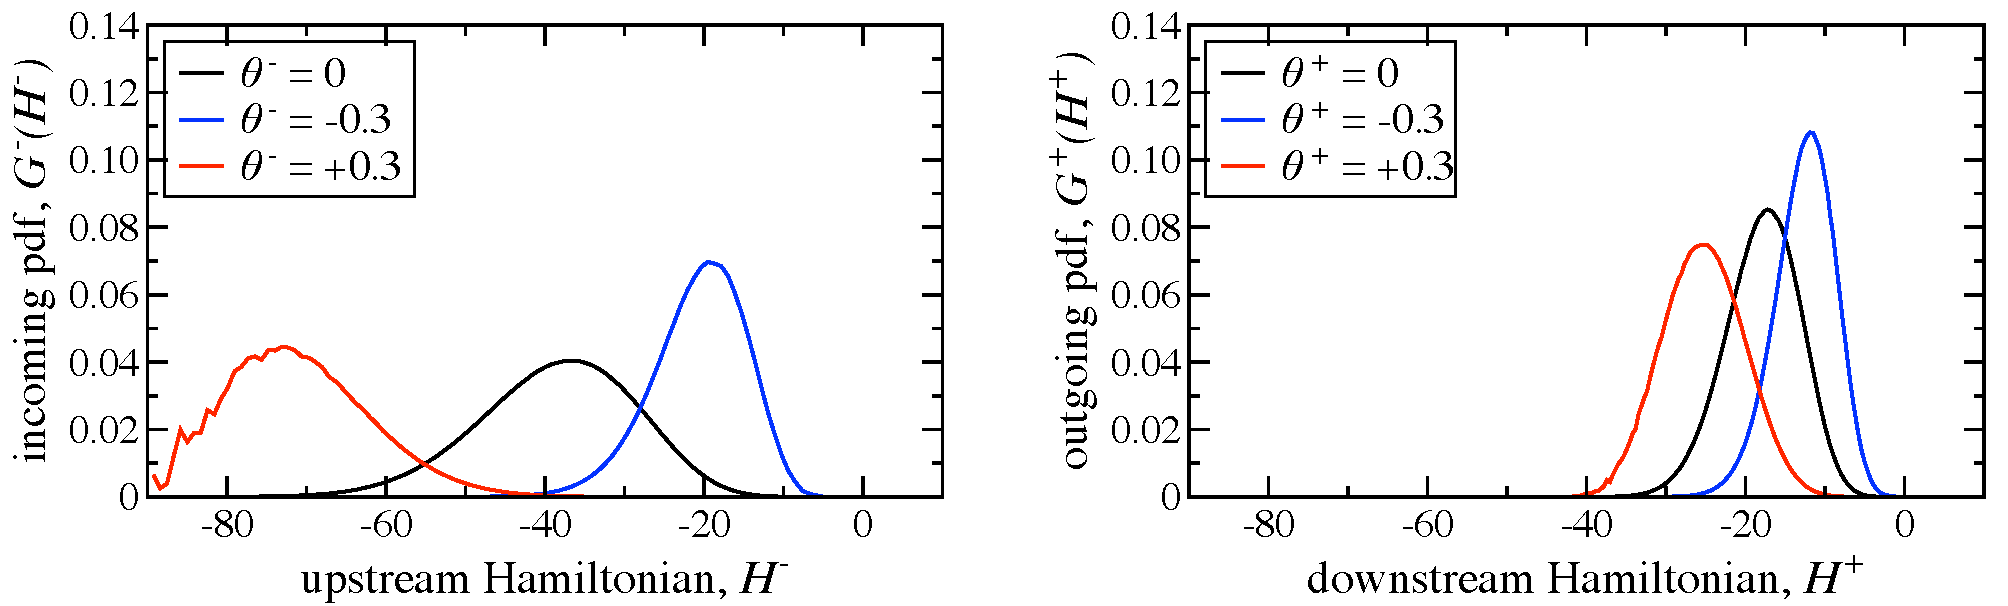
\includegraphics[width = 0.8 \textwidth]{Hist1}
\caption{Left: Sampling $H^-$ from the incoming Gibbs distribution $G^-$ with three different inverse temperatures $\theta^-$ (see legend). Right: Sampling the $H^+$ from an outgoing distribution $G^+$ with the same inverse temperatures.
In these tests, $\Lambda = 10$, $E_0 = 1$, $\lambda = 1$, $D_0 = 0.6$, and the number of samples is $1 \times 10^7$.}
\label{Hist1}
\end{center}
\end{figure}
 %^^^^^^^^^^^^^^^^^^^^^^^^^^^^^^%

%^^^^^^^^^^^^^^^^^^^^^^^^^^^^^^%
\begin{figure}[p]%[htbp]
\begin{center}
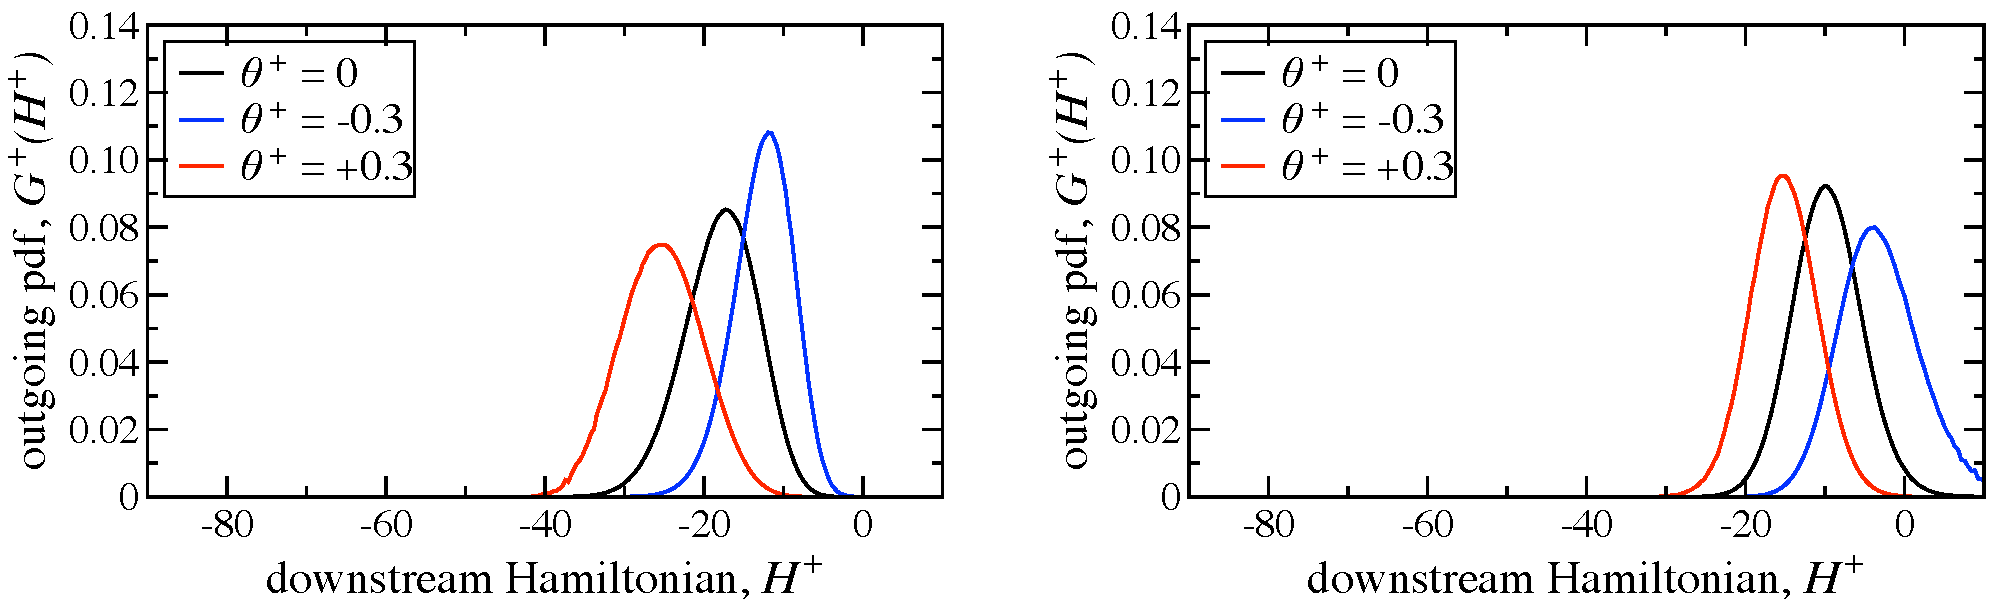
\includegraphics[width = 0.8 \textwidth]{Hist2}
\caption{Sensitivity to changes in $D_0$.
Left: Downstream histogram with $D_0 = 0.6$ (same as in Fig.~\ref{Hist1}). Right: Same with $D_0 = 0.4$. Notice the histogram changes significantly.
}
\label{Hist2}
\end{center}
\end{figure}
 %^^^^^^^^^^^^^^^^^^^^^^^^^^^^^^%

%^^^^^^^^^^^^^^^^^^^^^^^^^^^^^^%
\begin{figure}[p]%[htbp]
\begin{center}
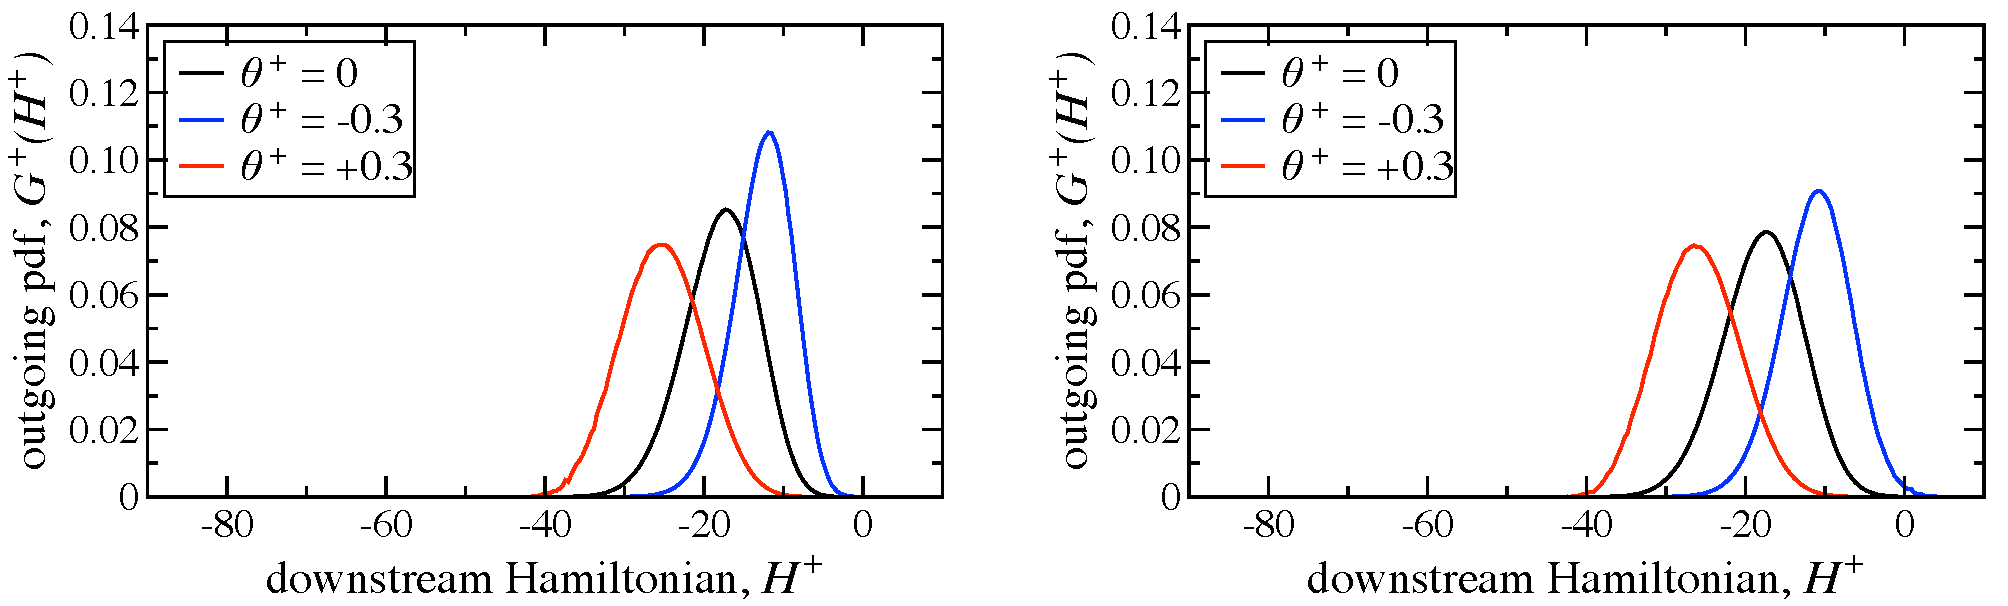
\includegraphics[width = 0.8 \textwidth]{Hist3}
\caption{Sensitivity to changes in the energy $E_0$.
Left: Downstream histogram with $E_0 = 1$ (same as in Fig.~\ref{Hist1}). Right: Same with $E_0 = 4$. Notice a slight change in the histogram.}
\label{Hist3}
\end{center}
\end{figure}
 %^^^^^^^^^^^^^^^^^^^^^^^^^^^^^^
 
 Next, in Figs.~\ref{microup0}--\ref{microdn3}, we examine various aspects of the microstates under given Gibbs distributions with possibly non-zero inverse temperatures. For this task, we need to use the acceptance/rejection algorithm described in Section \ref{sec_accrej}. In these tests, we again fix $\Lambda = 10$.
 
 First, Fig.~\ref{microup0} shows features of the microstate with zero inverse temperature (i.e.~the microcanonical distribution). The left panel shows a histogram of the displacement $u$ (in physical space). Notice the histogram is symmetric and resembles a Gaussian distribution. The right panel shows the $\mean{\abs{\uhat_k}}$ versus wavenumber $k$, which illustrates how the energy is distributed amongst the modes. Notice that the energy is evenly distributed amongst modes in this case, i.e.~a equidistribution of energy.
 
 In Fig.~\ref{microup3} we show the same plots but with $\theta^- = -0.3$. The histogram of $u$ is shown on the left. While this histogram still appears nearly symmetric, close examination reveals a slight positive skewness. The right shows $\mean{\abs{\uhat_k}}$. Notice that, in this case of negative inverse temperature, the spectrum is decidedly tilted, with less energy present in the higher modes.
 
 Figure \ref{microdn3} shows the same plots for the {\em downstream} distributions with $\theta^+ = -0.3$. Here, we have not enforced the statistical matching condition \eqref{statmatch}; we simply chose a value of $\theta^+$. First, notice that the histogram of $u$ shows a definite positive skewness. This observation is consistent with the main finding in the experiments! Second, the spectrum is tilted as before, but the tilt is not as strong as it is upstream. Both of these observations are consistent with the weights of $H_3$ and $H_2$. Downstream, the weights strongly favor $H_3$. Therefore, to have a better chance of being selected from the distribution $\Gibbs^{+}$, it is more advantageous to have large skewness of $u$ than it is to have small variance of $u_x$.
  
  %^^^^^^^^^^^^^^^^^^^^^^^^^^^^^^%
\begin{figure}[p]%[htbp]
\begin{center}
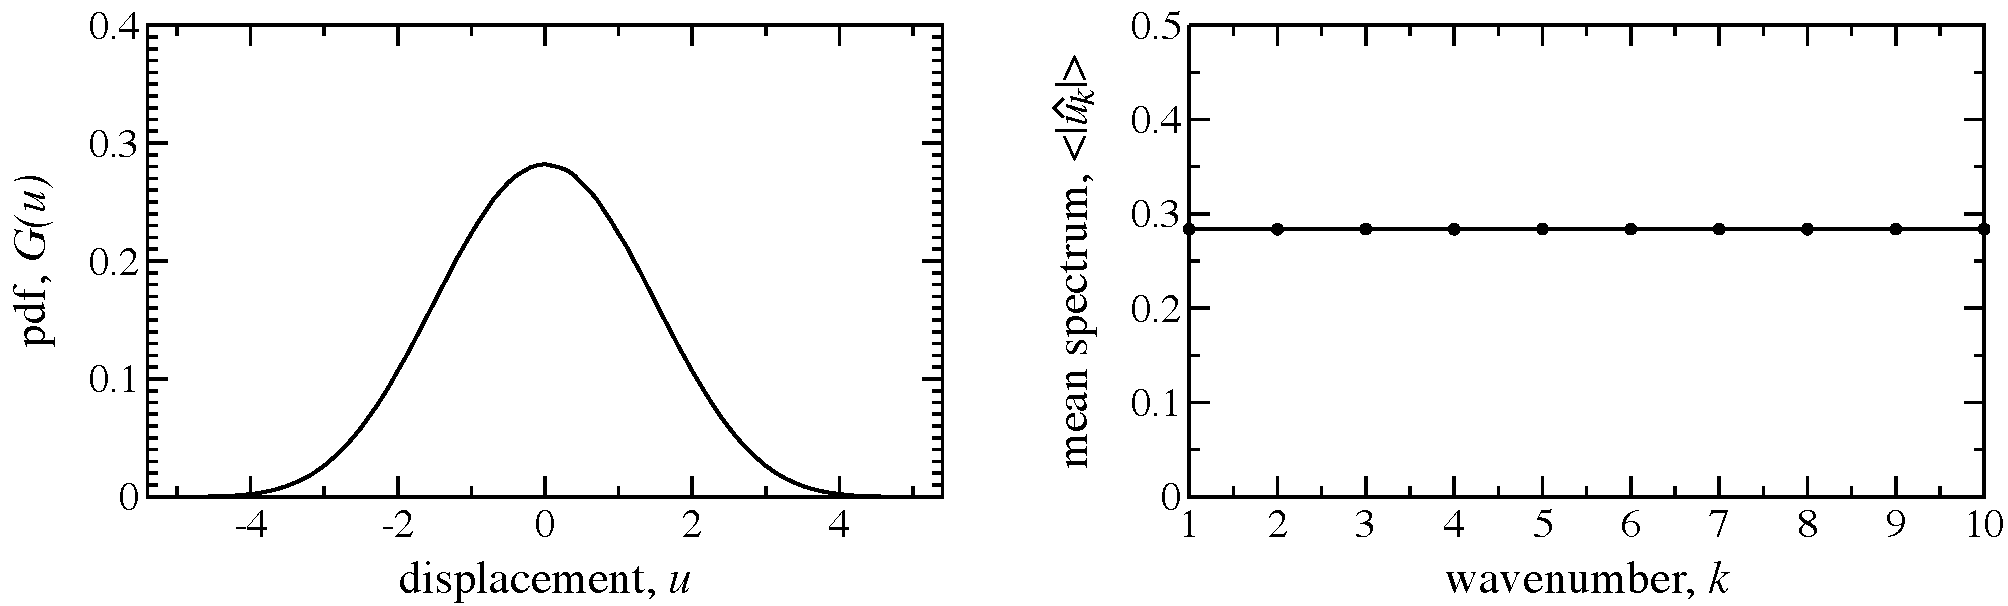
\includegraphics[width = 0.8 \textwidth]{microup0}
\caption{Sampling the upstream microstates with $\theta^- = 0$ (and $E_0 = 4$). Left: histogram of the surface displacement, $u^-$. Right: ensemble average of the spectrum, $\mean{\abs{\uhat_k}}$. Notice symmetric distribution of the displacement and the equipartition of energy amongst modes.}
\label{microup0}
\end{center}
\end{figure}
 %^^^^^^^^^^^^^^^^^^^^^^^^^^^^^^
 
 %^^^^^^^^^^^^^^^^^^^^^^^^^^^^^^%
\begin{figure}[p]%[htbp]
\begin{center}
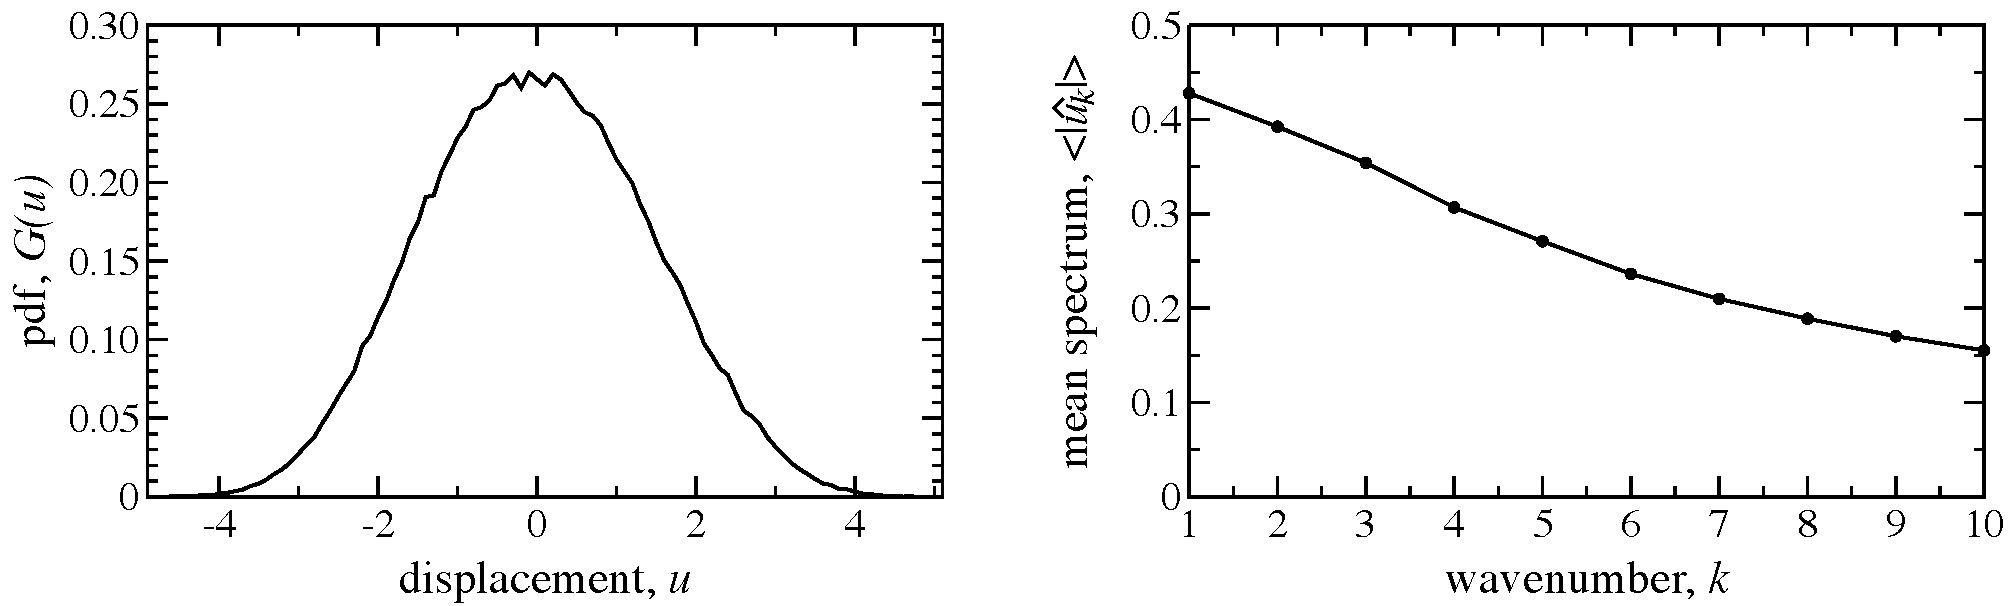
\includegraphics[width = 0.8 \textwidth]{microup3}
\caption{The upstream microstates with $\theta^- = -0.3$ (and $E_0 = 4$ as before). Notice the distinct tilt to the spectrum due to $\theta^- < 0$.}
\label{microup3}
\end{center}
\end{figure}
 %^^^^^^^^^^^^^^^^^^^^^^^^^^^^^^
 
  %^^^^^^^^^^^^^^^^^^^^^^^^^^^^^^%
\begin{figure}[p]%[htbp]
\begin{center}
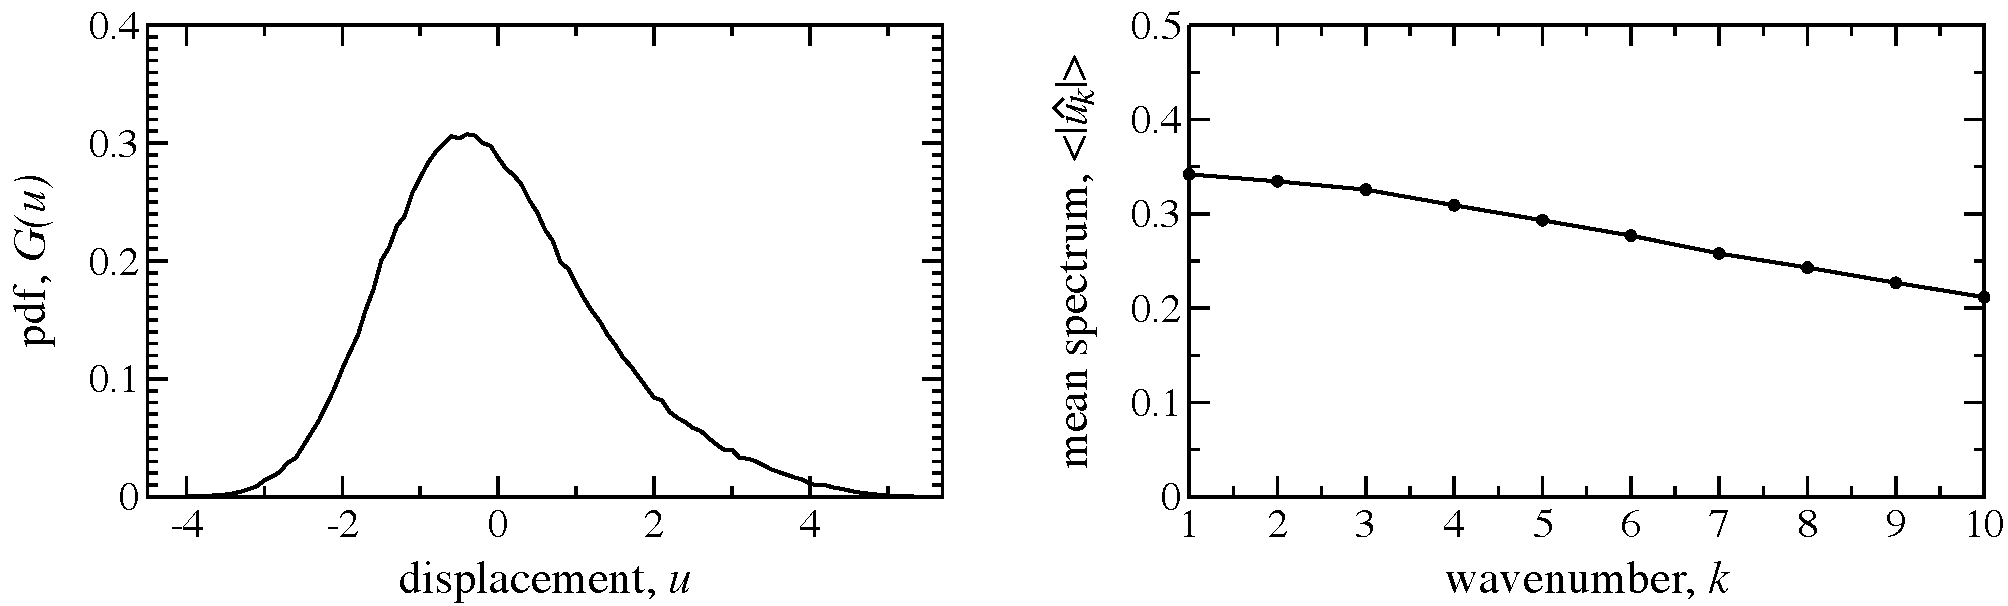
\includegraphics[width = 0.8 \textwidth]{microdn3}
\caption{Examination of the downstream microstates with $\theta^+ = -0.3$ and $D_0 = 0.5$ ($E_0 = 4$ as before). Notice the skewness of $u$! The spectrum is tilted, though not as much as it is upstream.}
\label{microdn3}
\end{center}
\end{figure}
 %^^^^^^^^^^^^^^^^^^^^^^^^^^^^^^
 
Now, figures \ref{match_theta}--\ref{match_micro} show results obtained by satisfying the matching condition \eqref{statmatch} using the algorithm described in \ref{sec_match}. In these tests, we use $\Lambda = 8$ and the provisional number of samples is $10^8$ (the number of accepted samples will be much lower). We also fix $E_0 = 4$ and $D_0 = 0.5$.

First, Fig.~\ref{match_theta} shows, for given values of $\theta^-$, the corresponding values of $\theta^+$ as determined by the matching condition. For one, $\theta^- = 0$ corresponds to $\theta^+ = 0$ which is a good sanity check. Second, notice that the signs of $\theta^-$ and $\theta^+$ always agree, which is a good thing. The relationship is not a simply linear one, as the curvature is significant.
 
 Next, Fig.~\ref{matchH} shows upstream and downstream histograms of $H$ with the matching condition enforced. The black curve is the histogram of $\Gibbs^-(H^-)$, while the colored curves are histograms of $H+$. The red curve corresponds to $\Gibbs^-(H^+)$ and the blue to $\Gibbs^+(H^+)$. The matching condition says that the means of these two histograms should be the same, which can be verified visually. Notice, the main difference is that the downstream histogram $\Gibbs^+(H^+)$ is more spread out.
 
Figure \ref{match_micro} shows features of the underlying microstates. On the left, we show histograms of the displacement $u$, as we did in Figs.~\ref{microup0}--\ref{microdn3}, but this time {\em we have enforced the matching condition} \eqref{statmatch}. Notice the upstream $u$-histogram is nearly symmetric, while the downstream histogram is noticeable skewed in the positive direction! The right panel shows the ensemble-averaged spectrum $\mean{\abs{\uhat_k}}$. Both show a tilt in the spectrum, with the upstream tilt being more significant than downstream.

We remark that simulations have been performed with larger values of $\Lambda$, for example $\Lambda = 16$ and 20. For the provisional number of samples fixed, increasing $\Lambda$ does not drastically increase the computational time. However, the main downside to increasing $\Lambda$ is that the acceptance rate for the Gibbs distributions is substantially smaller, and therefore the statistics are less resolved.


%^^^^^^^^^^^^^^^^^^^^^^^^^^^^^^%
\begin{figure}%[htbp]
\begin{center}
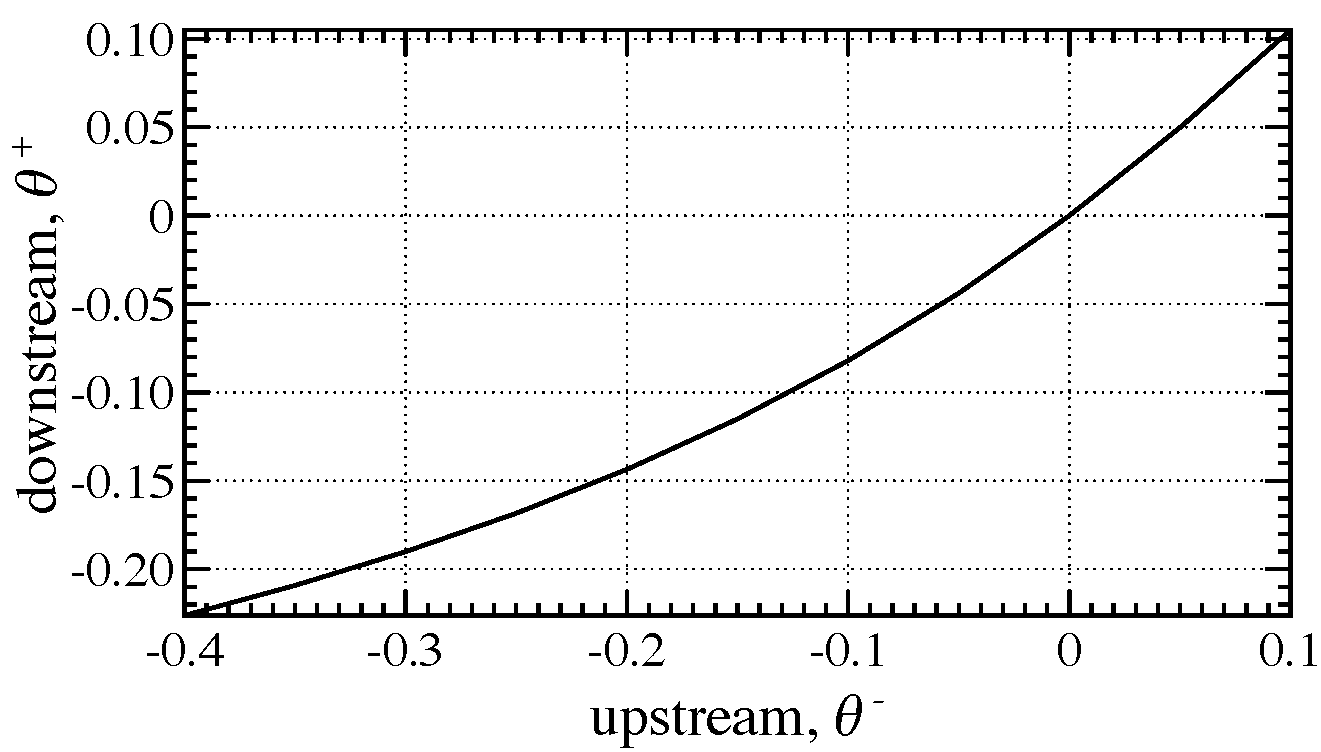
\includegraphics[width = 0.55 \textwidth]{match_theta}
\caption{For given values of $\theta^-$, we compute $\theta^+$ to satisfy the matching condition.}
\label{match_theta}
\end{center}
\end{figure}
 %^^^^^^^^^^^^^^^^^^^^^^^^^^^^^^
 
%^^^^^^^^^^^^^^^^^^^^^^^^^^^^^^%
\begin{figure}%[htbp]
\begin{center}
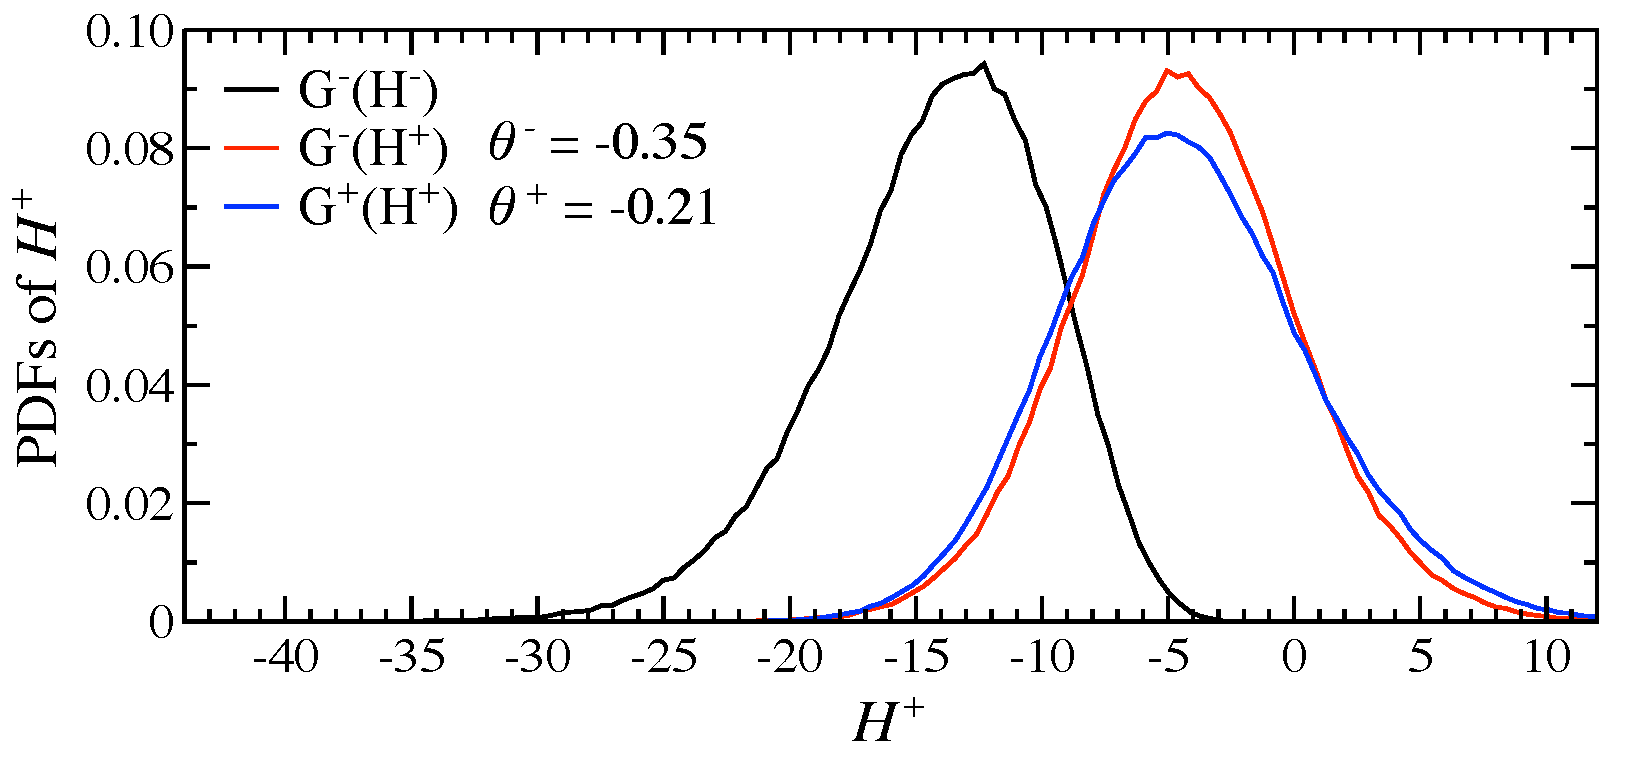
\includegraphics[width = 0.75 \textwidth]{matchH}
\caption{Histograms of $H^\pm$ under the two Gibbs measures $\Gibbs^{\pm}$ with the matching condition enforced.}
\label{matchH}
\end{center}
\end{figure}
 %^^^^^^^^^^^^^^^^^^^^^^^^^^^^^^
 
%^^^^^^^^^^^^^^^^^^^^^^^^^^^^^^%
\begin{figure}%[htbp]
\begin{center}
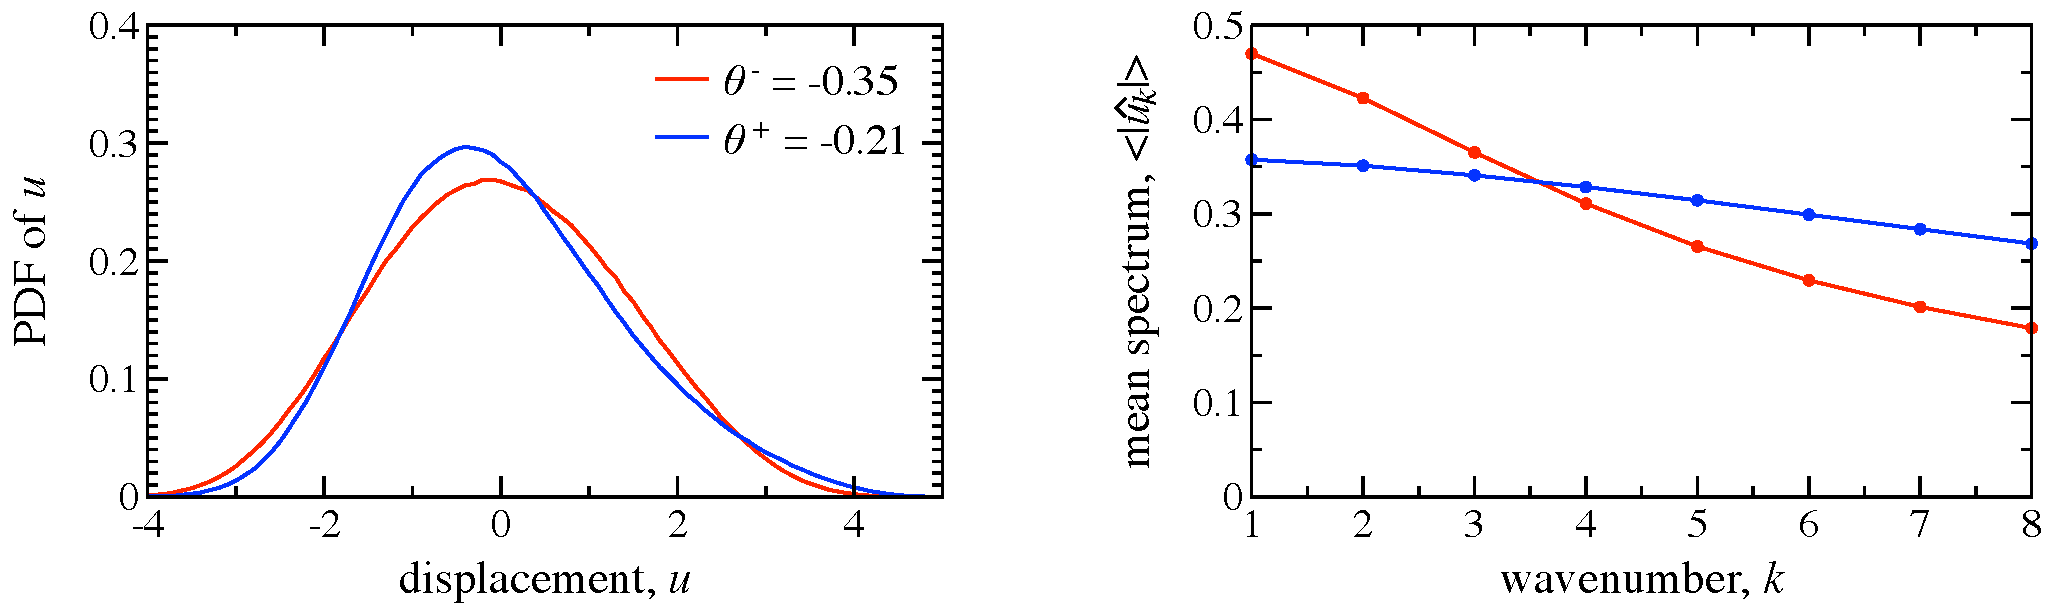
\includegraphics[width = 0.95 \textwidth]{match_micro}
\caption{Microstate features with the matching condition enforced. Left: the histogram of displacement $u$ upstream (red) and downstream (blue). Notice the downstream histogram has a definite positive skewness. Right: the ensemble-averaged spectra. Both spectra are tilted, with the upstream tilt being more significant.}
\label{match_micro}
\end{center}
\end{figure}
 %^^^^^^^^^^^^^^^^^^^^^^^^^^^^^^

\np
%%%%%%%%%%%%%%%%%%%%%%%%%%%%%%%%%%%%%%
%% Results
%%%%%%%%%%%%%%%%%%%%%%%%%%%%%%%%%%%%%%
\section{Big-time results}

Now lets do some more serious runs with larger $\Lambda$. The major challenge is that the acceptance rate plummets as $\Lambda$ grows, meaning that we either have to take many more samples or develop a smarter strategy. For now, we will do the first. To run more samples, I had to modify the organization of the code. I am still exploiting the ability to precompute a list of $H_3$ and $H_2$ values, but I cannot precompute and store the entire list at once because it will not fit in memory. So instead, I take several sweeps each with a manageable number of samples (usually about $10^7$).

Figure \ref{Lambda16Run} shows a run with $\Lambda = 16$, with $10^7$ samples per sweep and 200 sweeps for a total of $2 \times 10^9$ nominal samples. The main parameter to vary is the upstream inverse temperature $\theta^-$. More negative $\theta^-$ gives a more significantly skewed distribution of $u$, but also results in noisier statistics due to the lower acceptance rate. I therefore chose $\theta^- = -0.2$ since it gives a good balance of the two. The top panel of the figure shows $\theta^+$ as a function of $\theta^-$ and the histograms for $\theta^- = -0.2$. The bottom panel shows microstate information, including the pdf of displacement, $u$, and the spectrum. Notice the definite skew of the downstream displacement and the decay of both upstream and downstream spectra. For this run, the upstream acceptance rate was $0.01\%$ and the downstream rate was $0.008\%$. The total CPU time was about 33 hours.

%^^^^^^^^^^^^^^^^^^^^^^^^^^^^^^%
\begin{figure}%[htbp]
\begin{center}
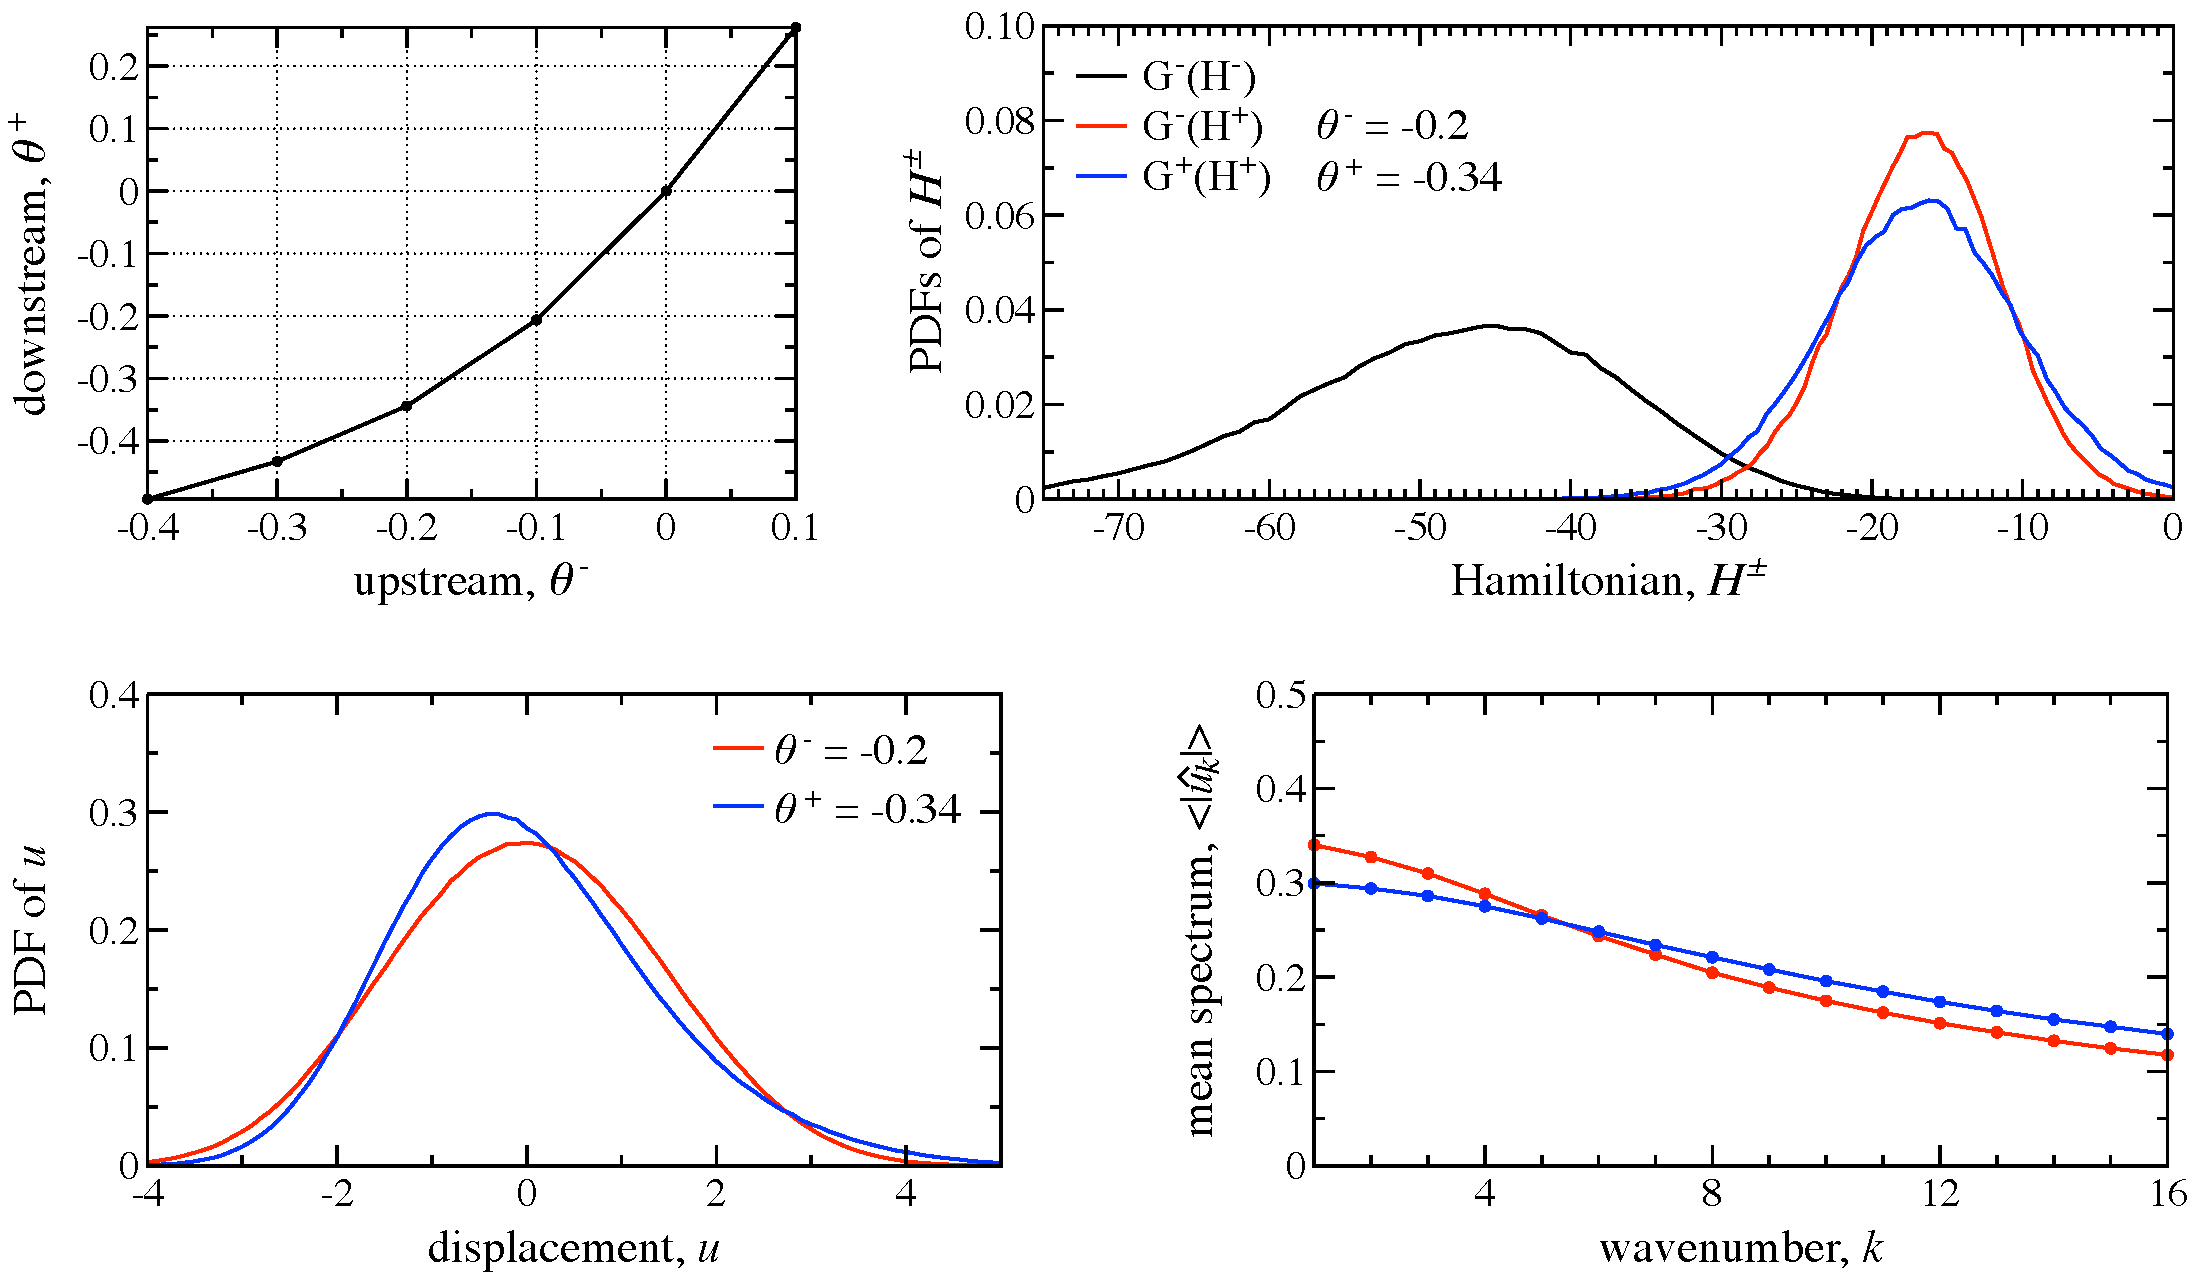
\includegraphics[width = 0.95 \textwidth]{Lambda16Run}
\caption{Big run with $\Lambda = 16$ and $2 \times 10^9$ nominal samples.}
\label{Lambda16Run}
\end{center}
\end{figure}
 %^^^^^^^^^^^^^^^^^^^^^^^^^^^^^^
 
\newpage
\newpage
\section{Experimental parameters}

Some relevant parameters from the experiment are given in the table.

% Table
%^^^^^^^^^^^^^^^^^^^^^^^^^^^^^^%
\begin{table}%[htbp]
\begin{center}
\caption{Some relevant experimental parameters} 
\vspace{0.3 pc}
\begin{tabular}{c l l}
\hline
\hspace{0.5pc} Symbol
\hspace{0.5pc} & Meaning 
\hspace{0.5pc} & Value \\
\hline
N/A		& Length of the experimental tank (in wave direction)	& 6 m	\\
$L_0$	& Width of the experimental tank	 (transverse)		& $L_0 = $ 20 cm	\\
$f_0$	& Dominant forcing frequency in experiments	& $f_0 = $ 2 Hz	\\
$\hm$	& Depth on deep side						& $\hm = 12.5$ cm \\
$\hp$	& Depth on shallow side					& $\hp = 3$ cm \\
$\lamm$	& Wavelength induced by 2 Hz forcing on deep side	& $\lamm = 38$ cm	\\
$\lamp$	& Wavelength induced by 2 Hz forcing on shallow side	& $\lamp = 25$ cm	\\
\hline
\end{tabular}
\end{center}
\end{table}
 %^^^^^^^^^^^^^^^^^^^^^^^^^^^^^^%
 


\begin{comment}
% Majda's notes typed up
\section{Deterministic model for waves over abrupt depth change}

The surface-displacement is denoted $u(x,t)$.

Modeling assumptions
\begin{enumerate}
\item Waves in a narrow channel (width $L_0$) are nearly unidirectional and $2 \pi L_0$ periodic (purely a mathematical idealization, not realistic I believe). Where $L_0 < \lambda$, with $\lambda$ a characteristic wavelength. As seen in the table, this later assumption is reasonable since $L_0 / \lamm \approx 0.5$
\item The role of the paddle forcing is to generate a state with `zero momentum', $M = \intt u \, dx = 0$ (this assumption is strongly supported by experimental measurements pointwise!) and with some given energy $E_0 = \frac{1}{2} \intt u^2 \, dx$ (not an assumption, just a statement). Here, $E_0$ is a function of the strength of the paddle forcing.
\item Assume a Galerkin truncation of $u(x,t) \approx u_{\Lambda}(x,t)$, where $\Lambda$ (fixed) will probably be 20 or 30.
\item The `time' coordinate $t$  corresponds physically to a downstream spatial coordinate (i.e.~$X \approx \eps x$ in Johnson's notation). The abrupt depth change (ADC) corresponds to $t = t_0$ or $T_{ADC}$.
\end{enumerate}
\end{comment}


\bibliographystyle{plain}
\bibliography{Notesbib}

\end{document}
